\chapter{Implementacja algorytmów}
Środowiskiem implementacji algorytmów jest ARDUINO 1.8.7 w wersji na system operacyjny Mac OS Mojave w wersji 10.14.
\section{Opis implementacji wybranych funkcji startowych}
W programie została użyta biblioteka dostarczona przez firmę Pololu do czujnika QRT-8RC QTRSensors.h w wersji 3.1.0.\cite{QRT} Do poprawnego działania czujnika zalecana jest kalibracja, która odbywa się zaraz po uruchomieniu robota.
Do odczytu wartości wykorzystywana jest funkcja:
\begin{lstlisting}[language=C]
    void qtrrc.read(sensorValues);
\end{lstlisting}
następnie za pomocą własnej funkcji:
\begin{lstlisting}[language=C]
    int QRT_ktory_widzi();
\end{lstlisting}
wyznaczany jest czujnik, który znajduje się nad linią.
\\
\\
W celu uruchomienia czujnika ultradźwiękowego US-015  wykonano sekwencje:
\begin{itemize}
    \item pin $TRIG$ ustawiony na stan niski;
    \item opóźnienie 2\si{\micro}s;
    \item pin $TRIG$ ustawiony na stan wysoki;
    \item opóźnienie 10\si{\micro}s;
    \item pin $TRIG$ ustawiony na stan niski.
\end{itemize}
\begin{figure}[H]
\centering
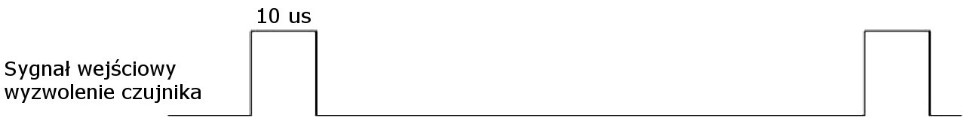
\includegraphics[width=0.9\textwidth]{inzynierku/img/sekwencja}
\caption{\label{fig:sekwencja}Sekwencja uruchomienia czujnika ultradźwiękowego.}
\end{figure}
Do sterowania silnikami zostały napisane trzy bliźniacze funkcje.
\begin{itemize}
    \item do sterowania lewym kołem
    \begin{lstlisting}[language=C]
    void stepperRotate_L(float rotation, float rpm);
    \end{lstlisting}
    \item do sterowania prawym kołem
    \begin{lstlisting}[language=C]
    void stepperRotate_P(float rotation, float rpm);
    \end{lstlisting}
    \item do sterowania dwoma kołami na raz -- jazda do przodu bądź do tyłu
    \begin{lstlisting}[language=C]
    void stepperRotate_S(float rotation, float rpm);
    \end{lstlisting}
\end{itemize}
Wszystkie wyżej wymienione funkcje przyjmują argumenty $rotation$ oraz $rpm$, które określają następująco ilość obrotów oraz prędkość obrotów.
W celu jazdy do przodu na pin $DIR$ należy podać sygnał wysoki, natomiast przy jeździe do tyłu stan niski.

\section{Opis algorytmu}
Działanie rozpoczyna się od kalibracji czujników wykrywania linii. Następnie przeprowadzana jest próba wykrycia przeszkody, jeśli owa zakończy się negatywnie, to robot próbuje podążać po linii. Podążanie po linii trwa dopóty robot nie natrafi na przeszkodę, gdzie ocenia którą stroną może ją ominąć, bądź zgłasza brak możliwości minięcia. Po ominięciu przeszkody kontynuuje jazdę po linii wyszukując następną przeszkodę powracając do fazy podążania po linii. Dokładny algorytm przedstawiony jest na rysunku \ref{fig:schemat_blokowy}.
\section{Graf algorytmu}
\begin{figure}[H]
\centering
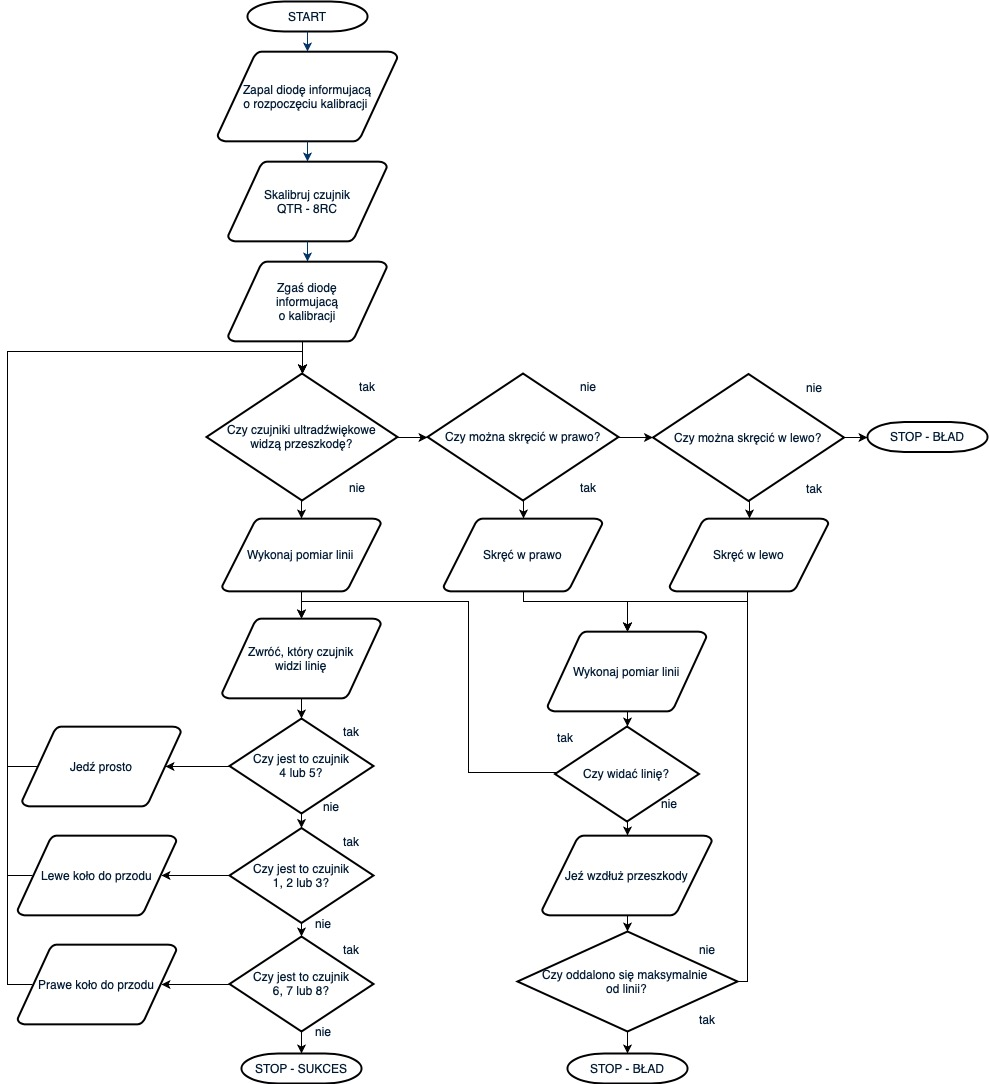
\includegraphics[width=\textwidth]{inzynierku/img/diagram}
\caption{\label{fig:schemat_blokowy}Schemat blokowy sterowania.}
\end{figure}